% 图 D.1 无限大平板的退磁场：(a) 磁化平行板面无磁极 (b) 垂直磁化产生磁极 (c) 退磁场 H_d
\documentclass[tikz,border=5pt]{standalone}
\usetikzlibrary{arrows.meta}
\usepackage{amsmath}
\usepackage{bm}
\usepackage{fontspec}
\setmainfont{Times New Roman}
\begin{document}
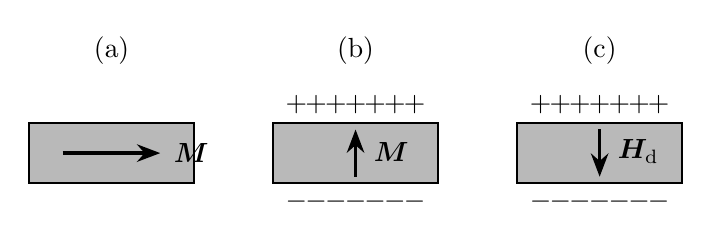
\begin{tikzpicture}[line width=0.8pt,>=Stealth]
\tikzset{slab/.style={fill=gray!55,draw=black,line width=0.8pt},
  varrow/.style={line width=1.2pt,->}}
% ---------- (a) M in plane ----------
\draw[slab] (-1.05,-0.38) rectangle (1.05,0.38);
\draw[varrow] (-0.62,0) -- (0.62,0);
\node[right] at (0.66,0) {$\bm{M}$};
\node at (0,1.30) {(a)};
% ---------- (b) M perpendicular, surface poles ----------
\begin{scope}[shift={(3.1,0)}]
  \draw[slab] (-1.05,-0.38) rectangle (1.05,0.38);
  \draw[varrow] (0,-0.30) -- (0,0.30);
  \node[right] at (0.10,0.02) {$\bm{M}$};
  \foreach \i in {0,...,6}{
    \node at (-0.75+0.25*\i,0.62) {$+$};
    \node at (-0.75+0.25*\i,-0.62) {$-$};}
  \node at (0,1.30) {(b)};
\end{scope}
% ---------- (c) demagnetizing field ----------
\begin{scope}[shift={(6.2,0)}]
  \draw[slab] (-1.05,-0.38) rectangle (1.05,0.38);
  \draw[varrow] (0,0.30) -- (0,-0.30);
  \node[right] at (0.10,0.02) {$\bm{H}_{\mathrm{d}}$};
  \foreach \i in {0,...,6}{
    \node at (-0.75+0.25*\i,0.62) {$+$};
    \node at (-0.75+0.25*\i,-0.62) {$-$};}
  \node at (0,1.30) {(c)};
\end{scope}
\end{tikzpicture}
\end{document}
